\documentclass[11pt,a4paper,finnish,oneside]{article}
\usepackage[utf8]{inputenc}     % Linux
%\usepackage[ansinew]{inputenc} % Windows 
\usepackage[T1]{fontenc}
\usepackage[finnish]{babel}
\usepackage[left=4cm,right=4cm,top=3cm,bottom=3cm]{geometry}
\usepackage{graphicx}
\usepackage{color}
\usepackage{epstopdf}
\usepackage[table]{xcolor}


\usepackage{subfig}



\sloppy
\definecolor{lightgray}{gray}{0.5}
\setlength{\parindent}{0pt}

\begin{document}
\begin{titlepage}  
\title{Graduaiheiden hallintajärjestelmä}
\author{(tsoha)}
\date{\today}
\maketitle    
\tableofcontents
\end{titlepage}    


\section{Johdanto}

\begin{par}
Hyvä graduaihe on monen toimijan keskinäisen koordinaation tuote. Graduaiheiden hallintajärjestelmä on luotu helpottamaan tätä koordinaatiota. Järjestelmä mahdollistaa opiskelijoiden ja ohjaajien selvittää, millaisia graduja on tehty, tai työn alla, ja kenen ohjauksessa. Nämä tiedot taas auttavat aiheiden ja ohjaajien etsinnässä, ja mm. päällekkäisyyksien välttämisessä.
\end{par}\vspace{1em}

\begin{par}
Ohjaaja lisää opiskelijan kanssa gradunteon aloittamisesta sovittuaan gradun aiheen järjestelmään, ja voi sen jälkeen muokata sitä halunsa mukaan. Ohjaaja myös luokitelee aiheen johonkin/joihinkin yleistasoiseen luokkaan, ja liittää siihen tietoja sen edistymisestä. Näistä tiedoista osa on ainoastaan ohjaajien käytettävissä.
\end{par}\vspace{1em}

\begin{par}
Järjestelmä toteutetaan tietojenkäsittelytieteen laitoksen users-palvelimella Tomcat- tai Apache-palvelimen alla. Alustajärjestelmän on tuettava PHP -ohjelmointikieltä ja järjestelmän käyttäjän selaimen javascriptiä. Käytettävän tietokannan on oltava PostgreSQL olio-relaatiotietokannan.
\end{par}

\section{Järjestelmän käyttäjät}
\subsection{Käyttötapauskaavio}


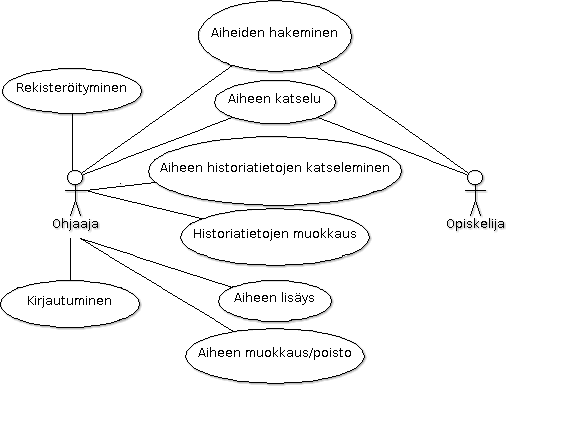
\includegraphics [width=6in]{useCase1.png}
\vspace{2em}

\subsection{Käyttäjäryhmät}
\begin{par}
\begin{description}
\item[Opiskelijalla]tarkoitetaan käytännössä ketä tahansa henkilöä, jota kiinnostaa tietää, millaisia graduja on tehty ja/tai tekeillä. Nämä henkilöt ovat potentiaalisia tai aktuaalisia opiskelijoita (tai heidän edustajiaan).
\item[Ohjaaja] on laitoksen graduohjaaksi hyväksymä henkilö, jolla on ollut/ on tällä hetkellä graduja ohjattavanaan, ja jonka ohjaajan ominaisuudessaan tarvitsee merkitä järjestelmään graduaiheita sekä päivittää niitten tietoja.
\end{description}
\end{par}
\subsection*{Käyttötapauskuvaukset}

\begin{par}

\subsubsection{Opiskelijan käyttötapaukset}

\begin{description}
  \item[Aiheiden hakeminen]\hfill\\Opiskelija hakee graduaiheita erityisalan tai ohjaajan perusteella. Hakutuloksena otsikoita sekä vuosilukuja.
  \item[Aiheen katselu]\hfill\\Opiskelija katsoo graduaiheeseen liittyvät tiedot, jotka hänen on mahdollista nähdä. 
\end{description}

\subsubsection{Ohjaajan käyttötapaukset}

\begin{description}
  \item[Aiheen lisäys]\hfill\\Ohjaaja lisää (yhteistyössä opiskelijan kanssa) graduaiheen, jonka on ottanut ohjattavakseen, liittäen siihen tiedon sen tekijästä sekä siihen liittyvistä eriyisaloista. Otsikko ja suunniteltua sisältöä valaiseva kuvaus.

  \item[Aiheen muokkaus/poisto]\hfill\\Ohjaaja muokkaa aiheen otsikkoa, kuvausta tai muita sen tietoja. Ohjaaja voi myös poistaa aiheen.

  \item[Aiheen historiatietojen katseleminen]\hfill\\Ohjaaja katsoo aiheeseen liittyviä historiatietoja. Ajankohtia kuten graduseminaarin suorittamisaika, gradun tarkastukseenjättämisaika jne. Ohjaajien tekemiä muistiinpanoja.
  
    \item[Aiheen historiatietojen muokkaus/lisäys/poisto]\hfill\\Ohjaaja muokkaa, lisää tai poistaa historiatietoja. 
  
\end{description}
Muita tapauksia: Kirjautuminen, rekisteröityminen, aiheiden haku, aiheen katselu.

\end{par}\vspace{1em}
\section{Järjestelmän tietosisältö}
\subsection{Käsitemalli}
\begin{center}
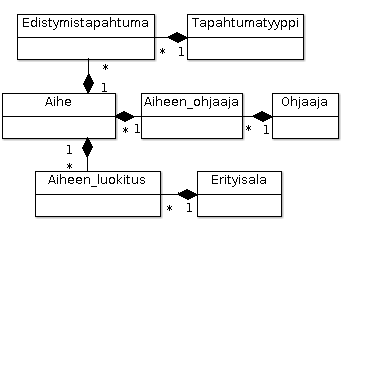
\includegraphics [width=4in]{infoContent1.png}
\end{center}
\subsection{Tietokohteiden kuvaukset}
    \begin{tabular}{ | p{3cm} | p{3cm} | p{6cm} |}
    \multicolumn{3}{l}{\textbf{Edistymistapahtuma}} \\ \hline
    {\small Attribuutti} & {\small Arvojoukko} & {\small Kuvailu}\\ \hline
    Aika & Päiväys & Tapahtuman ajankohta\\ \hline
    Merkitsijä & Ohjaajat & Tapahtuman merkinnyt ohjaaja \\ \hline
    Kommentti & Merkkijono, rajaton pituus & Kommentti, jossa lisätietoa tapahtumasta \\\hline
    \multicolumn{3}{l}{} \\

    \end{tabular}
Graduaiheeseen liittyvä historiatapahtuma, kertoo gradun edistymisestä. Graduaiheeseen voi liittyä useita tapahtumia, mutta tapahtumaan vain yksi graduaihe. Kuhunkin tapahtumaan liittyy tapahtumatyyppi sekä ohjaaja. Ohjaaja voi liittää tapahtumaan kommentin.

\vspace{2em}
    \begin{tabular}{ | p{3cm} | p{3cm} | p{6cm} |}
    \multicolumn{3}{l}{\textbf{Tapahtumatyyppi}} \\ \hline
    {\small Attribuutti} & {\small Arvojoukko} & {\small Kuvailu}\\ \hline
    Nimi & Merkkijono, max. 90 merkkiä & Edistymistapahtuman tyyppi\\ \hline
    \multicolumn{3}{l}{} \\

    \end{tabular}
Merkityksellinen tapahtuma gradun edistymisessä, esim. graduseminaarin päättyminen, gradun tarkastettavaksi jättö ja valmistuminen.

\vspace{2em}
    \begin{tabular}{ | p{3cm} | p{3cm} | p{6cm} |}
    \multicolumn{3}{l}{\textbf{Aihe}} \\ \hline
    {\small Attribuutti} & {\small Arvojoukko} & {\small Kuvailu}\\ \hline
    Otsikko & Merkkijono, max. 300 merkkiä & Graduaihetta kuvaava otsikko\\ \hline
    Kuvaus & Merkkijono, max 3000 merkkiä & Otsikkoa täsmentävä kuvaus \\ \hline
    Opiskelijanumero & Kokonaisluku, 9 numeromerkkiä & Tekijän opiskelijanumero \\\hline
    Nimi & Merkkijono, max. 80 merkkiä & Tekijän nimi \\\hline
    Luotu & Päiväys & Aiheen luontiajankohta\\\hline
    Luoja & Ohjaajat & Aiheen luonut ohjaaja\\\hline
    Linkki & verkko-osoite & Linkki valmiin gradun tietoihin\\\hline
    
    \multicolumn{3}{l}{} \\

    \end{tabular}
Aihe on keskeinen tietokohde graduaiheiden hallintajärjestelmässä. Aiheeseen liittyy historiatapahtumia sekä yksi tai useampia erityisaloja. Jokainen aihe on jonkun ohjaajan luoma. Gradulla voi olla useita ohjaajia.

\vspace{2em}
    \begin{tabular}{ | p{3cm} | p{3cm} | p{6cm} |}
    \multicolumn{3}{l}{\textbf{Ohjaaja}} \\ \hline
    {\small Attribuutti} & {\small Arvojoukko} & {\small Kuvailu}\\ \hline
    Etunimi & max. 40 merkkiä & Ohjaajan etunimi\\ \hline
    Sukunimi & max. 40 merkkiä & Ohjaajan sukunimi\\ \hline
    Salasana & Merkkijono max. 100 merkkiä & Salasana kirjautumista varten \\ \hline    
    Sähköposti & Merkkijono max. 80 merkkiä & Ohjaajan s-postiosoite \\ \hline
    \multicolumn{3}{l}{} \\

    \end{tabular}
Laitoksen graduohjaajaksi hyväksymä henkilö. Ohjaajalla voi olla monta gradua ohjattavanaan.

\vspace{2em}
    \begin{tabular}{ | p{3cm} | p{3cm} | p{6cm} |}
    \multicolumn{3}{l}{\textbf{Tutkimusala}} \\ \hline
    {\small Attribuutti} & {\small Arvojoukko} & {\small Kuvailu}\\ \hline
    Nimi & max. 90 merkkiä & Tutkimusalan nimi\\ \hline
    \multicolumn{3}{l}{} \\

    \end{tabular}
Yksi gradu voi liittyä useaan tutkimusalaan, ja tutkimusala useaan graduun.

\vspace{20em}
\section{Relaatiotietokantakaavio}

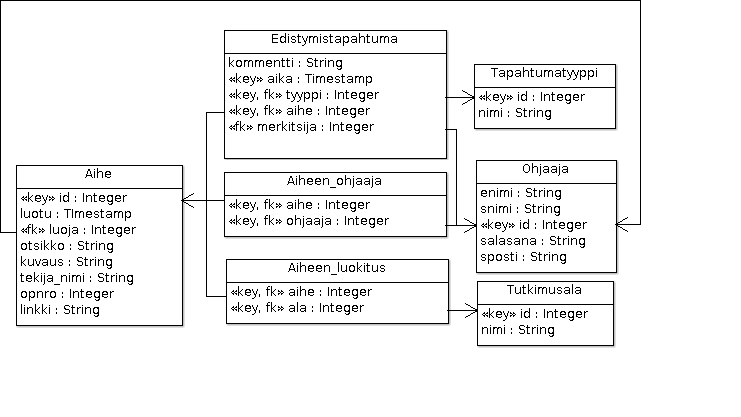
\includegraphics [width=7in]{classDiagram1.png}
\vspace{2em}


\end{document}
    
